\documentclass[14pt]{extarticle} 
\usepackage{amsmath,mathtools,amsfonts,amsthm,amssymb,hyperref}
\usepackage{wasysym,geometry,bussproofs,latexsym,parskip,bookmark}
\usepackage{mathtools,float}
\newtheorem{defn}{Definition}
\newtheorem{thm}{Theorem}
\newtheorem{claim}{Claim}
\newtheorem{lemma}{Lemma}
\newcommand{\dps}{\displaystyle}
\hypersetup{colorlinks,allcolors=blue,linktoc=all}
\geometry{a4paper} 
\geometry{margin=0.5in}
\title{Math for CS 2015/2019 solutions to ``In-Class Problems Week 12, Fri. (Session 30)''}
\author{https://github.com/spamegg1}
\begin{document}
\maketitle
\tableofcontents

\section{Problem 1}
Sally Smart just graduated from high school. She was accepted to three reputable colleges.

With probability 4/12, she attends Yale.

With probability 5/12, she attends MIT.

With probability 3/12, she attends Little Hoop Community College.

Sally is either happy or unhappy in college.

If she attends Yale, she is happy with probability 4/12.

If she attends MIT, she is happy with probability 7/12.

If she attends Little Hoop, she is happy with probability 11/12.

\subsection{(a)}
A tree diagram to help Sally project her chance at happiness is shown below. On the diagram, fill in the edge probabilities, and at each leaf write the probability of the corresponding outcome.

\begin{figure}[ht!]
\centering
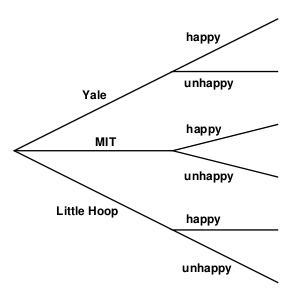
\includegraphics[scale=0.75]{happy.png}
\end{figure}

\begin{proof}
Just copy the numbers from above!
\end{proof}

\subsection{(b)}
What is the probability that Sally is happy in college?

\begin{proof}
Pr[happy] = Pr[Yale] $\cdot$ Pr[Yale \& happy] + Pr[MIT] $\cdot$ Pr[MIT \& happy] + Pr[LH] $\cdot$ Pr[LH \& happy]

Pr[happy] = $\dps\frac{4}{12}\cdot\frac{4}{12} + \frac{5}{12}\cdot\frac{7}{12} + \frac{3}{12}\cdot\frac{11}{12} = \frac{84}{144} = \frac{7}{12}$
\end{proof}

\subsection{(c)}
What is the probability that Sally attends Yale, given that she is happy in college?

\begin{proof}
By Bayes' Theorem and part (b):

Pr[Yale $|$ happy] = $\dps\frac{Pr[\text{happy} \,|\, \text{Yale}] \cdot Pr[\text{Yale}]}{Pr[\text{happy}]} = \frac{(4/12)\cdot(4/12)}{7/12} = \frac{16}{84} = \frac{4}{21}$
\end{proof}

\subsection{(d)}
Show that the event that Sally attends Yale is not independent of the event that she is happy.

\begin{proof}
Pr[Yale] $\dps = \frac{4}{12} \neq \frac{4}{21} = $ Pr[Yale $|$ happy]

Therefore by definition of independence, the event that Sally attends Yale is not independent of the event that she is happy.
\end{proof}

\subsection{(e)}
Show that the event that Sally attends MIT is independent of the event that she is happy.
\begin{proof}
By Bayes' Theorem:

Pr[MIT $|$ happy] = $\dps\frac{Pr[\text{happy} \,|\, \text{MIT}] \cdot Pr[\text{MIT}]}{Pr[\text{happy}]} = \frac{(7/12)\cdot(5/12)}{7/12} = \frac{5}{12}$

Therefore:

Pr[MIT] $\dps = \frac{5}{12} = \frac{5}{12} = $ Pr[MIT $|$ happy]

Therefore by definition of independence, the event that Sally attends MIT is independent of the event that she is happy.
\end{proof}

\section{Problem 2}
Suppose you flip three fair, mutually independent coins. Define the following events:

Let $A$ be the event that the first coin is heads.

Let $B$ be the event that the second coin is heads.

Let $C$ be the event that the third coin is heads.

Let $D$ be the event that an even number of coins are heads.

\subsection{(a)}
Use the four step method to determine the probability space for this experiment and the probability of each of $A, B, C, D$.

\begin{proof}
The tree is a binary tree with depth 3 and 8 leaves. The successive levels branching to show whether or not the successive events $A$, $B$, $C$ occur. By definition of fair and independent, each branch out of a vertex is equally likely to be followed. So the probability space has as outcomes the eight length-3 strings of H’s and T’s, each of which has probability $(1/2)^3 = 1/8$. Each of the events $A, B, C, D$ is true in four of the outcomes and hence has probability 1/2.
\end{proof}

\subsection{(b)}
Show that these events are not mutually independent.
\begin{proof}
$$
Pr[A\cap B\cap C\cap D] = 0 \neq (1/2)^4 = Pr[A]\cdot Pr[B]\cdot Pr[C]\cdot Pr[D]
$$
\end{proof}

\subsection{(c)}
Show that they are 3-way independent.

\begin{proof}
Because the coin tosses are mutually independent, we know:

$$
Pr[A\cap B\cap C] = Pr[A]\cdot Pr[B]\cdot Pr[C]
$$

What remains is to check that equality holds for the other subsets of three events: $\{A, B, D\}, \{A, C, D\}$, and $\{B, C, D\}$. By symmetry, again, we need only check one, say the first one.
$$
Pr[A \cap B \cap D] = Pr[HHT] = \frac{1}{8} = Pr[A]\cdot Pr[B]\cdot Pr[D]
$$
So the three events $\{A, B, D\}$ are independent. We conclude that all four events are three-way independent.
\end{proof}

\section{Problem 3 (Graphs, Logic \& Probability)}
Let $G$ be an undirected simple graph with $n > 3$ vertices. Let $E(x, y)$ mean that $G$ has an edge between vertices $x$ and $y$, and let $P(x, y)$ mean that there is a length 2 walk in $G$ between $x$ and $y$.

\subsection{(a)}
Write a predicate-logic formula defining $P(x, y)$ in terms of $E(x, y)$.
\begin{proof}
If there is a length 2 walk between $x$ and $y$ then there is a third vertex $z$ such that there is an edge between $x$ and $z$, and there is an edge between $z$ and $y$. Therefore:
$$
P(x,y) \Coloneqq \exists z(z \neq x \text{ AND } z \neq y \text{ AND } E(x,z) \text{ AND } E(z,y))
$$
If we assume that self-loops are not allowed, then $z \neq x$ and $z \neq y$ are forced, so we can remove them:
$$
P(x,y) \Coloneqq \exists z(E(x,z) \text{ AND } E(z,y))
$$
\end{proof}

For the following parts (b)-(d), let $V$ be a fixed set of $n > 3$ vertices, and let $G$ be a graph with these vertices constructed randomly as follows: for all distinct vertices $x, y \in V$, independently include edge $\langle x - y\rangle$ as an edge of $G$ with probability $p$. In particular, Pr[$E(x, y)] = p$ for all $x \neq y$.

\subsection{(b)}
For distinct vertices $w, x, y$ and $z$ in $V$, circle the event pairs that are independent.

\subsubsection{}
1. $E(w, x)$ versus $E(x, y)$

\begin{proof}
They are independent, as explained in the definition of $G$ above.
\end{proof}

\subsubsection{}
2. $[E(w, x)$ AND $E(w, y)]$ versus $[E(z, x)$ AND $E(z, y)]$

\begin{proof}
They are independent. Each event has probability $p^2$, and their intersection has probability $p^4$. 
\end{proof}

\subsubsection{}
3. $E(x, y)$ versus $P(x, y)$

\begin{proof}
They are independent. $P(x, y)$ involves the existence of a third vertex $z$ different than $x, y$. The events $E(x,y)$, $E(x,z)$, $E(y,z)$ are three-way independent for every $z \neq x,y$. 
\end{proof}

\subsubsection{}
4. $P(w, x)$ versus $P(x, y)$

\begin{proof}
???
\end{proof}

\subsubsection{}
5. $P(w, x)$ versus $P(y, z)$

\begin{proof}
???
\end{proof}

\subsection{(c)}
Write a simple formula in terms of $n$ and $p$ for Pr[NOT $P(x, y)$], for distinct vertices $x$ and $y$ in $V$.

Hint: Use part (b), item 2.
\begin{proof}
Write $V = \{x, y, z_1, \ldots, z_{n-2}\}$. Then NOT $P(x, y)$ is
$$
\text{NOT } ([E(x, z_1) \text{ AND } E(z_1, y)] \text{ OR } \ldots \text{ OR } [E(x, z_{n-2}) \text{ AND } E(z_{n-2}, y)])
$$
which is equivalent to
$$
\text{NOT}[E(x, z_1) \text{ AND } E(z_1, y)] \text{ AND } \ldots \text{ AND } \text{NOT}[E(x, z_{n-2}) \text{ AND } E(z_{n-2}, y)]
$$
Each NOT $[E(x, z_i)$ AND $E(z_i, y)]$ has probability $1-p^2$ and they are all independent of each other by part (b) item 2, so the AND chain of these events has probability $(1-p^2)\cdot \ldots \cdot (1-p^2) = (1-p^2)^{n-2}$.

\end{proof}

\subsection{(d)}
What is the probability that two distinct vertices $x$ and $y$ lie on a three-cycle in $G$? Answer with a simple expression in terms of $p$ and $r$, where $r \Coloneqq$ Pr[NOT$(P(x, y))$] is the correct answer to part (c).

Hint: Express $x$ and $y$ being on a three-cycle as a simple formula involving $E(x, y)$ and $P(x, y)$.

\begin{proof}
$x$ and $y$ are on a 3-cycle iff $E(x,y)$ AND $P(x,y)$. By part (b), item 3, $E(x,y)$ is independent of $P(x,y)$. So
$$
Pr[x, y \text{ are on a 3-cycle}] = Pr[E(x,y)] \cdot Pr[P(x,y)] = p^2 \cdot (1-r)
$$
\end{proof}

\section{Problem 4 (Supplemental Problem)}
Let $A, B, C$ be events. For each of the following statements, prove it or give a counterexample.

\subsection{(a)}
If $A$ is independent of $B$, then $A$ is also independent of $\overline{B}$.

\begin{proof}
Notice $A \cap \overline{B} = A - (A \cap B)$, so
$$
\begin{array}{rclr}
Pr[A \cap \overline{B}]&=&Pr[A] - Pr[A\cap B]&\text{(by above)}\\
&=&Pr[A] - Pr[A]\cdot Pr[B]&\text{(since $A$ and $B$ are independent)}\\
&=&Pr[A]\cdot (1- Pr[B])&\\
&=&Pr[A] \cdot Pr[\overline{B}]&
\end{array}
$$
\end{proof}

\subsection{(b)}
If $A$ is independent of $B$, and $A$ is independent of $C$, then $A$ is independent of $B \cap C$. Hint: Choose $A, B, C$ pairwise but not 3-way independent.

\begin{proof}
The experiment is 2 independent coin flips, letting $A$ be “the 1st flip is heads”, $B$ the “the 2nd flip is heads,” $C$ is “odd number of heads.” Then $A$ is independent of $B$, $A$ is independent of $C$, but $A$ is not independent of $B \cap C$ because
$$
Pr[A \,|\, B \cap C] = \frac{Pr[A \cap (B \cap C)]}{Pr[B \cap C]} = \frac{Pr[\emptyset]}{Pr[TH]} = 0 \neq 1/2 = Pr[A]
$$
\end{proof}

\subsection{(c)}
If $A$ is independent of $B$, and $A$ is independent of $C$, then $A$ is independent of $B \cup C$. Hint: Part (b).

\begin{proof}
The experiment is 2 independent coin flips, letting $A$ be “the 1st flip is heads”, $B$ the “the 2nd flip is heads,” $C$ is “odd number of heads.” Then $A$ is independent of $B$, $A$ is independent of $C$, but $A$ is not independent of $B \cup C$ because
$$
Pr[A \,|\, B \cup C] = \frac{Pr[A \cap (B \cup C)]}{Pr[B \cup C]} = \frac{Pr[HH, HT]}{Pr[HH, TH, HT]} = 2/3 \neq 1/2 = Pr[A]
$$
\end{proof}

\subsection{(d)}
If $A$ is independent of $B$, and $A$ is independent of $C$, and $A$ is independent of $B \cap C$, then $A$ is independent of $B \cup C$.

\begin{proof}
We can use Conditional Inclusion/Exclusion principle, followed by the regular Inclusion/Exclusion principle:
$$
\begin{array}{rclr}
Pr[B \cup C \,|\, A]&=&Pr[B\,|\,A] + Pr[C\,|\,A] - Pr[B\cap C \,|\, A]&\text{(by Cond. Incl/Excl)}\\
&=&Pr[B] + Pr[C] - Pr[B \cap C]&\text{(by independence)}\\
&=&Pr[B \cup C]& \text{(by regular Incl/Excl)}
\end{array}
$$
\end{proof}
\end{document}
